%!TEX root = ../../report.tex

\subsubsection{Cellular Automaton} % (fold)
\label{ssub:cellular_automaton}


It's a model of a system of cells within a grid with a determined shape, each of this cells can be on one of a finite set of states. It evolves during a finite amount of time steps with a set of simple rules according with the state of the neighbouring cells.
The neighbourhood of the cell can be defined in many different ways, the most common is the use of the adjacent cells.

Starting from a line with zeros except the middle cell with one and the following set of rules:

\begin{figure}[htbp]
	\centering
	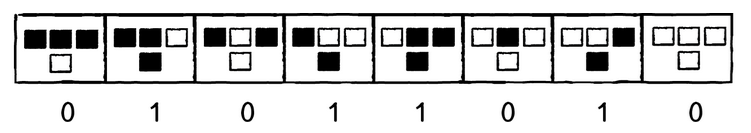
\includegraphics[width=0.85\textwidth]{img/Theory/Cellular_A/Rules.png}
	\caption{Example Production Rules\cite{Shiffman2012}}
	\label{fig:label}
\end{figure}



The Figure~\ref{fig:resultCA} image represents the evolution of one Cellular automaton over time.  In this case, each cell can have one of two states, black or white. Starting from a white line except the middle cell that is black and the presented set of rules.

\begin{figure}[htbp]
    \centering
    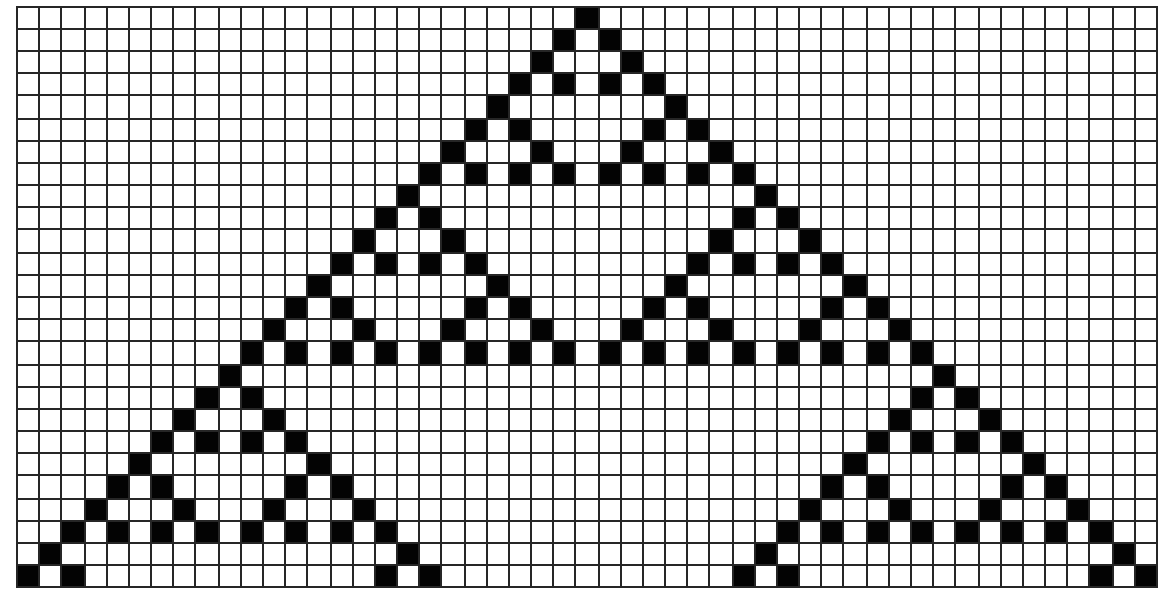
\includegraphics[width=0.85\textwidth]{img/Theory/Cellular_A/Result.png}
    \caption{Sierpiński Triangle}
    \label{fig:resultCA}
\end{figure}



In Figure~\ref{fig:resultCA} each line represents an iteration of the system with the application of the rules. With this set of rules a Sierpiński triangle is reproduced.


% subsubsection cellular_automaton (end)